\documentclass[a4paper]{article}

\usepackage[english]{babel}
\usepackage[utf8]{inputenc}
\usepackage{times}
\usepackage{amsmath}
\usepackage{amssymb}
\usepackage{graphicx}
\usepackage{subcaption}
\usepackage{float}
\usepackage[colorinlistoftodos]{todonotes}
\usepackage{hyperref}
\usepackage{listings}

\setlength{\parskip}{\baselineskip}%
\setlength{\parindent}{0pt}%
\frenchspacing

\lstset{
    frame=single,
    basicstyle=\footnotesize\ttfamily
}

\title{Experimental data transmission method using sound}

\author{FÁBIÁN Tamás László}

\date{\today}

\begin{document}
\maketitle

\section{Introduction}

A method for transmitting and receiving 20 bytes long data packets 
using sound is described. The method uses continuous-phase multiple frequency-shift keying (CPFSK), and a robust synchronization method. A Reed-Solomon code is used for forward error correction.

A software was written in the Python language for experimental and 
demonstration purposes. Scripts are provided to send and receive short 
text messages using the computer's audio devices, or to read/write the 
audio to/from data files. The files can be played back, or converted 
into more traditional audio formats using sox\cite{sox1}.

A framework was established to gauge the performance of the software. A 
script can generate random messages and save them into audio files with 
various levels of white noise. An other script then can be used to 
attempt decoding these files. Various statistics are shown after the 
script finished decoding the files.

Experiments show that this method can transmit data 99.9\% accurately 
at a carrier to noise ratio (CNR) of -11dB (or at about 10dB 
$E_b/N_0$) measured over 22.05 KHz bandwidth, and with 83.4\% accuracy 
at -12dB CNR (about 9dB $E_b/N_0$).

In real-world experiments using a small set of consumer-grade computer 
audio devices reliable data transfer could be achieved over 1 meter 
in a quiet room at quite low volume levels. Noisy environments mandate 
higher volume setting and/or shorter distances. Interference due to 
multipath propagation probably is the main performance bottleneck.

\section{Theory of Operation}

I provide a summary on the operation of the software. See the in-line
code documentation for implementation details.

\subsection{Modulation}

The data has to be transmitted and received with equipments designed to
produce and record audio. Since little was known about the working
environment, an Additive Gaussian White Noise (AGWN) channel was used
as the channel model. In real life however, it is likely that noise
bursts will occur frequently.

Audio sampling rate was determined to be 44.1KHz. This sampling rate 
along with 48KHz is the most frequently supported one, and 48KHz audio 
can easily be downsampled on devices only supporting that.

The channel properties were chosen so that the transmitting device 
could be a low-quality piezoelectric speaker. A carrier frequency of 
about 4KHz, and a maximum bandwidth of also 4KHz was determined. The 
bandwidth were kept lower than the carrier frequency, to prevent 
harmonics interfering with the reception, so the transmitter can drive 
the speaker with a square wave.

Using 44100 samples per second sampling rate, a 200 sample DFT will have
a bucket size of 220.5 Hz. To keep the modulation process simple, one
transmitted symbol will contain 4 bits, or half a byte of information.
To encode 4 bits, a symbol must communicate 16 separate states.

The modulation uses 17 frequencies in the form of $4410 + n*220.5$ Hz
where $n \in [0..16] \cap \mathbb{Z}$. About half of the time the
carrier ($n=0$) is transmitted, and no actual data is sent. This is for
synchronization. When this tone is off, one of the other 16 frequencies
($n \in [1..16] \cup \mathbb{Z}$) is transmitted, this is when data is
actually being transmitted. So instead of 16 symbols, a 17 symbol
alphabet is being used, out of which the carrier or zero symbol is used
for frame synchronization.

The carrier is turned on-off in a way so it can easily be found using 
correlation. The exact sequence of on-off states affect how easily it 
may be spotted by correlating a potentially noisy and arbitrary 
time-shifted signal with a known, clean synchronization sequence.

Good sync sequences were found using gradient descent with random 
restarts: essentially by checking random sequences, and looking for 
neighbors with increasingly better properties, until the process 
stuck in a local optimum, after which it is restarted from an other
random vector.

A total of 200 symbols are transmitted, out of those 108 are used to 
transmit data, and 92 used for synchronization only. Transmitting one 
frame takes about 0.907 seconds. \textbf{The effective bit rate is 
176.4bps.}

\subsection{Demodulation}

Demodulation begins by recording a chunk of audio longer than a single
frame. After normalizing the received data and correlating it with the
synchronization sequence, a decision is made whether there is a signal
present. The correlation will return the position where the sync signal
matches the audio the most.

Using the position information 108 DFTs at positions where the first
tone is off. The received power in each bin is observed, and a hard
decision is made about what symbol the particular 200-sample audio data
might encode. Only the DFTs encoding the 108 data nibbles are kept.

\subsection{Forward Error Correction}

A Reed-Solomon code RS(54,20) were chosen for forward error correction,
mainly because implementations were readily available, and of course
because of their good performance.

The error correcting code takes 20 byte payload, and produces a 54 byte
codeword. The code is capable of correcting 17 errors or 34 erasures.
Currently the software does not signal erasure towards the decoder,
but there are methods\cite{ft1} for doing so.

\section{The Software}

This section describes how the software should be operated to run
demonstrations and experiments.

\subsection{Prerequisites}

The demonstration software requires a functional Python 3.6 
installation, and a machine with enough resources. The following 
configuration \textit{before} Python installation is recommended:

\begin{itemize}
\item Intel Core i5 processor, or better
\item 4GB RAM
\item 6GB of free disk space
\item Speakers
\item Microphone
\item Ubuntu Linux 17.04 or newer is recommended, a recent Windows or
macOS should also work
\end{itemize}

It is recommended to install a Python distribution called Anaconda
\cite{ana1}. Anaconda a contains stable and fast Python build along
with several important libraries.

\subsection{Installation}

Anaconda 5.0.1 with Python 3.6 can be downloaded from:

\url{https://www.anaconda.com/download}.

There are installers for Linux, Windows and macOS operating system. Any 
of those systems should be able to run the demo software, but it had 
only been tested throughly on Ubuntu Linux "zesty" 17.04.

The scripts \texttt{send.py} and \texttt{receive.py} use 
\textit{pyaudio}, a Python binding for an audio library called 
\textit{portaudio}. The portaudio library (.so, .dll, or .dynlib) and 
header files need to be installed. The installation process differs 
across operating systems, and can be as simple as issuing a command 
(Linux and maxOS), or having to install Visual Studio and compile the 
library by hand (Windows)\footnote{This is why the .dll-s and headers 
bundled with the pyaudio Python library for Windows}.

\subsubsection{Installation on Ubuntu Linux "zesty" 17.04}

The \texttt{portaudio19-dev} package need to be installed with the 
package manager \texttt{apt}:

\begin{lstlisting}
$ sudo apt install portaudio19-dev
$ cd <path-to-demo-software>
$ pip install -r requirements.txt
\end{lstlisting}

\subsubsection{Installation on Apple macOS}

Portaudio need to be installed using \texttt{brew}:

\begin{lstlisting}
$ brew install portaudio
$ cd <path-to-demo-software>
$ pip install -r requirements.txt
\end{lstlisting}

\subsubsection{Installation on Microsoft Windows}

On Windows, the portaudio binaries are included in the pyaudio wheel, 
so separate installation should not be necessary (make sure 
\texttt{pip} and \texttt{python} are on the \texttt{PATH}):

\begin{lstlisting}
C:\> cd <path-to-demo-software>
C:\> pip install -r requirements.txt
\end{lstlisting}

\subsection{Usage}

The scripts \texttt{test-gen.py} and \texttt{text-score.py} can 
generate a large set of audio files, and run a decoding benchmark on 
them respectively. Any computer capable of running Python properly may 
be used to run the benchmark. Since the process involves generating
14000 files consuming about 1.2GB space, this should be done on a fast
machine.

The scripts \texttt{send.py} and \texttt{receive.py} use audio devices 
to play and record audio. They use the default system device, but they 
can set up to use any device with the \texttt{-d <number>} or 
\texttt{--device <number>} parameter. Use \texttt{devices.py} to view a 
list of audio devices.

All command examples assume Linux operating system, but they should 
work with no or only minor modifications on macOS and Windows too. 
Commands should be executed in the directory where the scripts are 
located.

\subsubsection{Listing audio devices}

The \texttt{devices.py} script shows a list of audio devices available. 
On some systems error messages may occur on the first few lines. These 
can be ignored.

Since \texttt{send.py} and \texttt{receive.py} are using the default 
audio device, this list will probably rarely be needed.

\newpage

\begin{lstlisting}
$ ./devices.py 
ALSA lib pcm.c:2495:(snd_pcm_open_noupdate) Unknown PCM cards.pcm.rear
ALSA lib pcm.c:2495:(snd_pcm_open_noupdate) Unknown PCM
cards.pcm.center_lfe
ALSA lib pcm.c:2495:(snd_pcm_open_noupdate) Unknown PCM cards.pcm.side
ALSA lib pcm_route.c:867:(find_matching_chmap) Found no matching
channel map
0 HDA Intel PCH: ALC898 Analog (hw:0,0)
1 HDA Intel PCH: ALC898 Digital (hw:0,1)
2 HDA Intel PCH: ALC898 Alt Analog (hw:0,2)
3 USB Audio CODEC: - (hw:1,0)
4 HDA NVidia: HDMI 0 (hw:2,3)
5 HDA NVidia: HDMI 1 (hw:2,7)
6 HDA NVidia: HDMI 2 (hw:2,8)
7 HDA NVidia: HDMI 3 (hw:2,9)
8 sysdefault
9 front
10 surround21
11 surround40
12 surround41
13 surround50
14 surround51
15 surround71
16 iec958
17 spdif
18 pulse
19 dmix
20 default
$
\end{lstlisting}

\subsubsection{Sending or saving messages}

The \texttt{send.py} script can send a message by playing the modulated
audio carrier on an audio device, or saving and audio file.

In it's simplest form it's just called with a short text to send:

\begin{lstlisting}
$ ./send.py test
CNR (dB):    inf
Eb/N0 (dB):  inf
Peak:        0.252437119188
$
\end{lstlisting}

The command always displays the estimated carrier to noise power ratio 
and $E_b/N_0$ in decibels. Since there is no noise added by default, 
both figures are displayed as being infinite.

Adding noise, distortion and saving the audio into a file:

\begin{lstlisting}
$ ./send.py -f test.s16 -c -11 -d 10000 test
CNR (dB):    -11.0397105534
Eb/N0 (dB):  9.92938957672
Peak:        0.742417642773
$
\end{lstlisting}

The files store a single audio channel at a sampling rate of 44100 KHz.
Each sample is a signed 16 bit little endian integer. The files contain
no header or any kind of metadata.

One can specify a string of hexadecimal digits to send with the 
\texttt{-x} or \texttt{--hex} flag:

\begin{lstlisting}
$ ./send.py -f test.s16 -c -11 -d 10000 -x \
  9d7133b7f07274a5be88a06f7b5ae2914822c008

CNR (dB):    -11.0397105534
Eb/N0 (dB):  9.92938957672
Peak:        0.742417642773
$
\end{lstlisting}

For a brief description of usage and parameters, issue 
\texttt{./send.py -h}.

\subsubsection{Receiving or loading messages}

The script \texttt{receive.py} can be used to load audio files, or 
decode audio read from an audio device in real-time. The test.s16 file 
created above can (very likely) be decoded with the following 
command:

\begin{lstlisting}
$ ./receive.py -f test.s16 -x
Got sync signal, decoding... 
DECODED: >>> 9d7133b7f07274a5be88a06f7b5ae2914822c008 <<<
End of data stream reached, terminating
$
\end{lstlisting}

Without the \texttt{-f} parameter the script listens on the default 
audio device. The \texttt{-x} flag is useful for printing arbitrary 
binary data. Without this flag the script tries to convert the received 
data to ASCII strings, and print that instead of hex digits. Call the 
script with the \texttt{-h} parameter to get a list of usable flags 
and parameters and their descriptions.

\subsubsection{Recording audio}

A short script is provided for Linux using the SoX command 
\texttt{rec}, and providing it with the necessary parameters, so only 
the file name has to be given:

\begin{lstlisting}
$ ./rec.sh test.s16

Input File     : 'default' (alsa)
Channels       : 1
Sample Rate    : 44100
Precision      : 16-bit
Sample Encoding: 16-bit Signed Integer PCM

In:0.00% 00:00:05.20 [00:00:00.00] Out:221k  [ -====|====- ]     Clip:0
Aborted.
$
\end{lstlisting}

The recording can be stopped by hitting CTRL+C. It is worth keeping an 
eye on the "Clip" indicator at the end of the last line. If this 
counter starts growing then the audio level is too high.

\subsubsection{Playing saved audio}

Playing audio is also handled by SoX via a Linux shell script:

\begin{lstlisting}
$ ./play.sh test.s16 

test.s16:

 File Size: 459k      Bit Rate: 706k
  Encoding: Signed PCM    
  Channels: 1 @ 16-bit   
Samplerate: 44100Hz      
Replaygain: off         
  Duration: 00:00:05.20  

In:100%  00:00:05.20 [00:00:00.00] Out:229k  [      |      ]     Clip:0    
Done.
$
\end{lstlisting}

\subsubsection{Generating test files}

The test set generator script will generate one thousand random test 
files for each CNR level. The tested levels are between and including
-14dB and -1 dB.

The \texttt{test-gen.py} script accepts no arguments, and calling it 
will start generating test files right away:

\begin{lstlisting}
$ ./test-gen.py 
  0%|                              | 5/14000 [00:01<1:06:18,  3.52it/s]
$
\end{lstlisting}

During test set generation a progress bar with the speed and ETA is 
displayed. Before generating a test set, make sure the \texttt{data} 
directory only contains a \texttt{.gitignore} file, and no *.s16 audio 
files. These are not removed automatically, and new files will have
different names every time.

Every file is exactly 1 second, or 44100 samples -- 88200 bytes -- 
long. The signal is right in the middle of every file at offset 2050.

\subsubsection{Scoring performance on a test file set}

The \texttt{test-score.py} script will read any .s16 files from the 
data directory and will attempt to demodulate and decode them. It will 
record any success or failure in finding the synchronization signal or 
decoding the actual message.

Before exiting, the script will print out a rather dense representation 
of the results. It looks like this:

\begin{lstlisting}
FILES:         {-5: 1000, -3: 1000, -4: 1000, -14: 1000, ...
GOOD DECODES:  {-5: 1000, -3: 1000, -4: 1000, -12: 834, ...
NO DECODES:    {-14: 1000, -13: 897, -12: 166, -11: 1}
BAD DECODES:   {}
GOOD SYNCS:    {-5: 1000, -3: 1000, -4: 1000, -14: 980, ...
BAD SYNCS:     {-13: 10, -14: 20, -12: 1, -11: 1}
BAD SYNC SET:  {2040, 2060}
\end{lstlisting}

Each line shows a metric. The number before the colons are specific CNR 
values, the number after the colons are the number of occurrences.

For example the ,,FILES'' line shows the number of files. It can be 
seen that for the CNR level of -5(dB) there were ,,1000'' files in the 
data directory.

It can also be seen that for levels -5, -3 and -4 ever file was decoded 
OK, and only 834 ,,GOOD DECODES'' were possible at CNR level -12.

,,NO DECODES'' counts files that could not be decoded at all, ,,BAD 
DECODES'' count files that could be decoded, but the results were 
different from the originally encoded data. ,,GOOD SYNCS'' show the 
number of files where the synchronization signal could be recovered 
with utmost precision. ,,BAD SYNCS'' counts ill-identified sync 
vectors. ,,BAD SYNC SET'' shows all the offsets where a sync vector was 
found, except the correct 2050 offset.

\subsubsection{Generating synchronization vectors}

The synchronization vector has to have a special property: it must have 
low aperiodic autocorrelation. Such vectors are rare, and long vectors 
are hard to find. The script \texttt{syncvec-search.py} tries to find 
such vectors using gradient descent with random restarts. This script 
was used design/development time, and can be used again if (when) 
changing the modulation becomes necessary.

\subsubsection{Observing saved audio waveforms and spectra}

A script named \texttt{scope.py} is provided for graphically displaying 
waveforms stored in s16 files. The script accepts a file name as a 
single mandatory positional parameter, and various flags that control 
what should be displayed. By default a simple waveform is displayed.

The following flags are available:

\begin{description}
\item[\texttt{-h}] Show help and exit.
\item[\texttt{-s}] Show spectrum.
\item[\texttt{-c}] Show correlation vector.
\item[\texttt{-w}] Show waterfall.
\item[\texttt{-o}] Offset: skip this many samples.
\item[\texttt{-y}] Synchronize: try to find a packet, cut it out, and.
  display only that
\end{description}

Some examples follow showing clean and noisy signals.

\begin{lstlisting}
$ ./scope.py clean.s16
...
$ ./scope.py noisy.s16
...
\end{lstlisting}

\begin{figure}[H]
    \centering
    \begin{subfigure}[b]{0.45\textwidth}
        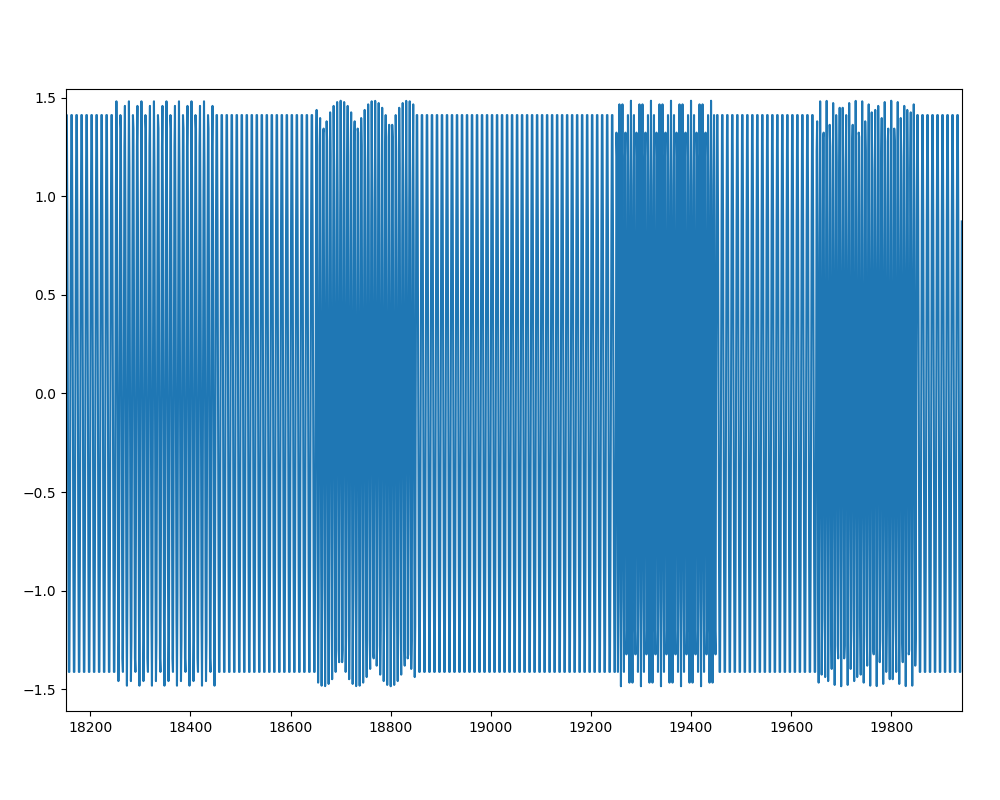
\includegraphics[width=\textwidth]{scope_clean.png}
        \caption{Clean waveform}
    \end{subfigure}
    \begin{subfigure}[b]{0.45\textwidth}
        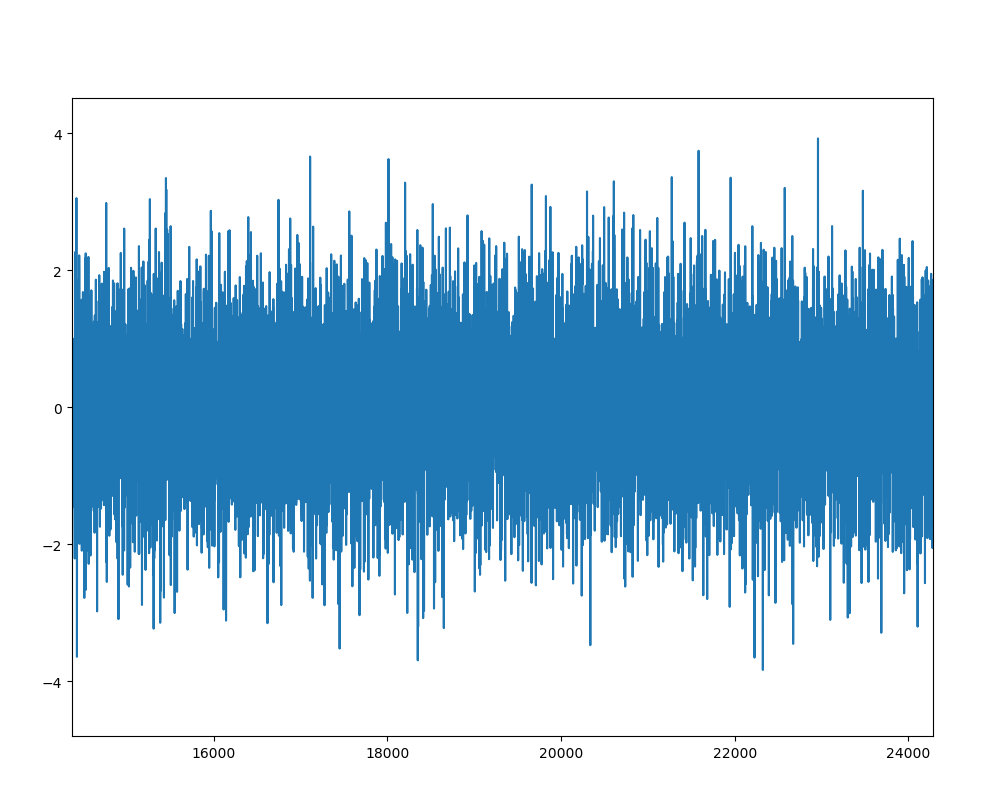
\includegraphics[width=\textwidth]{scope_noisy.png}
        \caption{Noisy waveform}
    \end{subfigure}
\end{figure}

\begin{lstlisting}
$ ./scope.py -s clean.s16
...
$ ./scope.py -s noisy.s16
...
\end{lstlisting}

\begin{figure}[H]
    \centering
    \begin{subfigure}[b]{0.45\textwidth}
        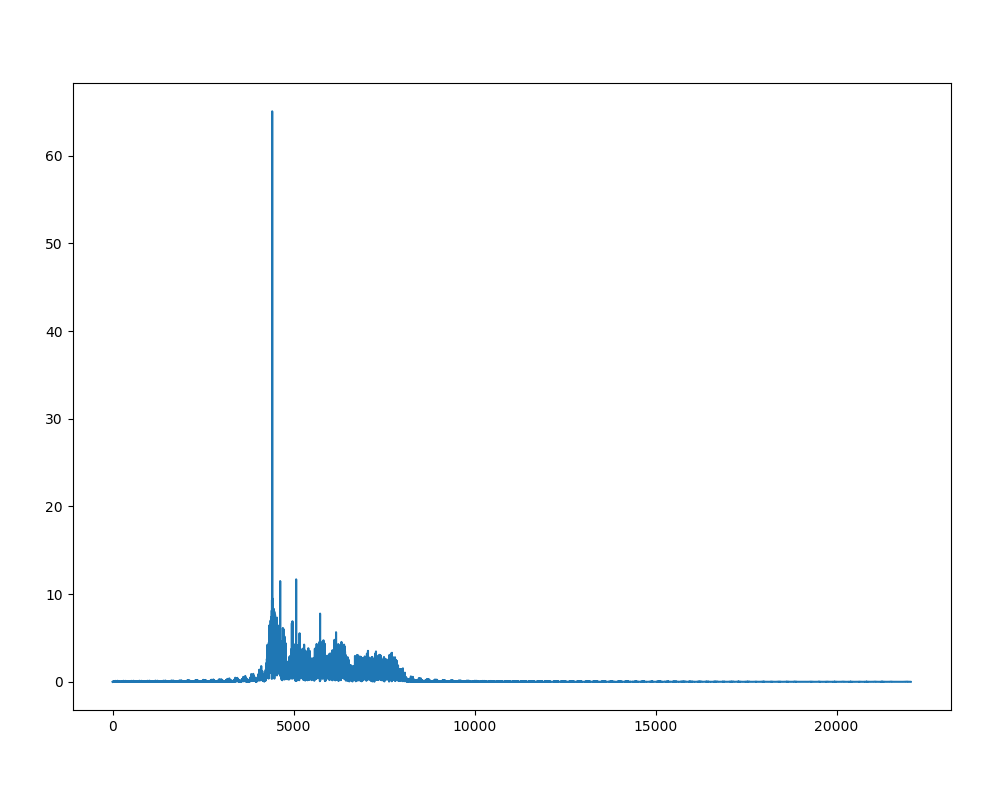
\includegraphics[width=1\textwidth]{dft_clean.png}
        \caption{Clean DFT}
    \end{subfigure}
    \begin{subfigure}[b]{0.45\textwidth}
        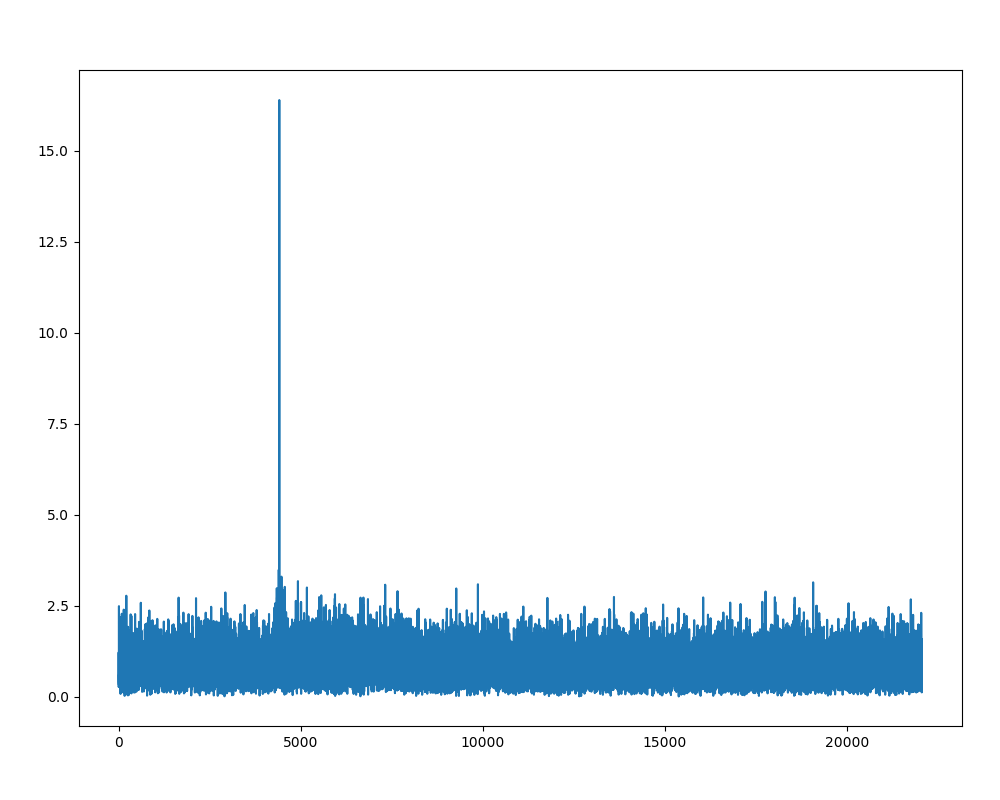
\includegraphics[width=1\textwidth]{dft_noisy.png}
        \caption{Noisy DFT}
    \end{subfigure}
\end{figure}

\begin{lstlisting}
$ ./scope.py -c clean.s16
...
$ ./scope.py -c noisy.s16
...
\end{lstlisting}

\begin{figure}[H]
    \centering
    \begin{subfigure}[b]{0.45\textwidth}
        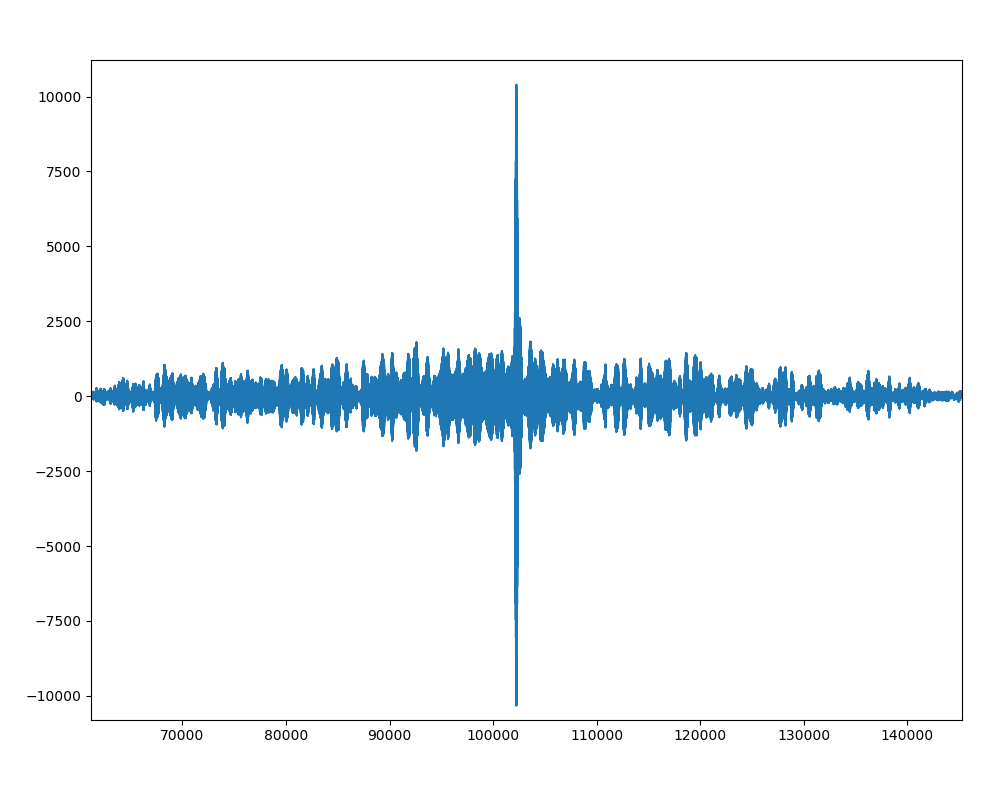
\includegraphics[width=1\textwidth]{correlation_clean.png}
        \caption{Correlation vector, clean signal}
    \end{subfigure}
    \begin{subfigure}[b]{0.45\textwidth}
        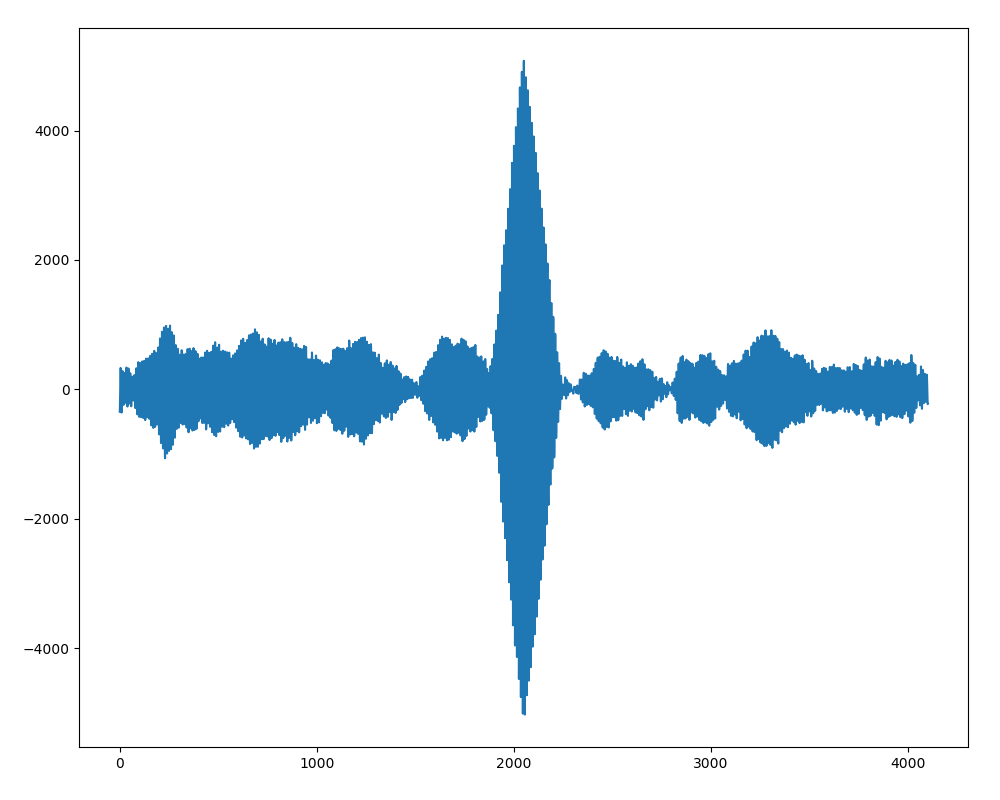
\includegraphics[width=1\textwidth]{correlation_noisy.png}
        \caption{Correlation vector, noisy signal}
    \end{subfigure}
\end{figure}

\begin{lstlisting}
$ ./scope.py -y -w clean.s16
...
$ ./scope.py -y -w noisy.s16
...
\end{lstlisting}

\begin{figure}[H]
    \centering
    \begin{subfigure}[b]{0.45\textwidth}
        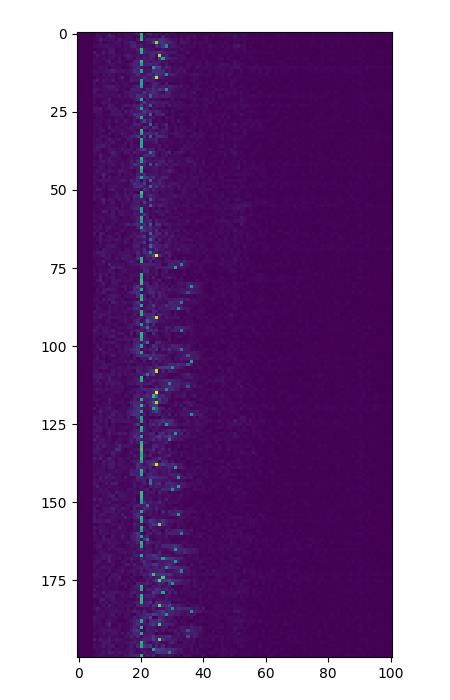
\includegraphics[width=1\textwidth]{waterfall_sync_clean.png}
        \caption{Clean signal, synchronized}
    \end{subfigure}
    \begin{subfigure}[b]{0.45\textwidth}
        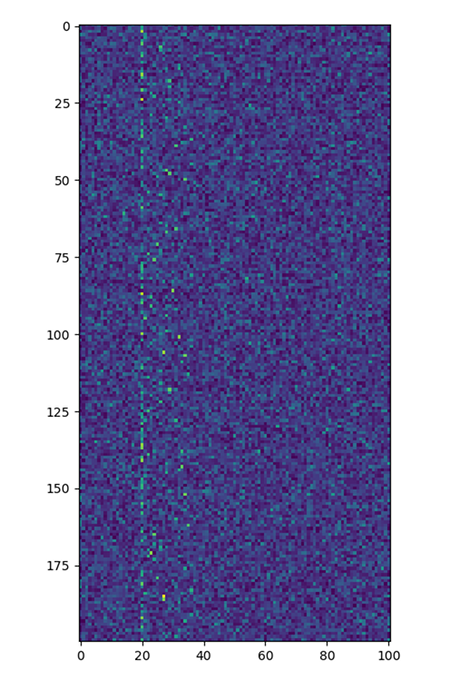
\includegraphics[width=1\textwidth]{waterfall_sync_noisy.png}
        \caption{Noisy signal, synchronized}
    \end{subfigure}
\end{figure}

\section{Experimental results}

A large number of simulations, and some real-world experiments were
conducted. These are described below.

\subsection{Real-World Experiments}

Real-world experiments in the given time frame could only yield a
modest number of data points. The following description focuses more on
usability and other practical aspects, and does not try to communicate
precise figures.

\subsubsection{Single PC setup}

A single desktop personal computer with a high quality speaker and 
microphone were used to test performance at the early stages of 
development.

\textbf{With this setup I could easily achieve reliable data transfer 
at distances slightly over 1 meter even when music played, or people 
were talking if the microphone and speaker were facing each other.}

Performance was heavily dependent on the microphone setup and volume 
setting. Too high volume causes clipping and destroys the signal, to 
low volume hides the signal in the noise of the recording equipment. If 
the microphone were facing in a direction other than the speaker, 
\emph{multipath propagation} was found to interfere with reception.

\subsubsection{Single notebook setup}

A single laptop computer was used to try and replicate the results. The 
notebook had a built-in microphone with lots of noise, since it was 
equipped with forced air cooling, and the fan was on most of the time.

The built-in microphone and the speaker were about 12cm close together. 
The received signals weren't as high quality as with the PC setup. This 
was due not to the distance, but to the fact that the speakers and the 
microphone were deliberately placed and insulated so that the audio 
feedback is as little as possible.

The microphone in this setup faces away from the speakers, and picks 
other sounds up easily, including the sound of the speakers bouncing
off objects, and arriving from the front. Because of this, the signal
gets back to the receiver multiple times with some delay.
This can easily confuse the demodulator.

\subsubsection{Notebook-PC setup}

To rule out any problem with the laptop's microphone and audio 
circuitry, several experiments were conducted with the PC set being the 
transmitter, and it being the receiver.

A performance similar to the PC-only setup were measured: signals could 
easily be picked up from about 1 meter even when the laptop's fan were 
on, or when some music or noise could be heard in the room. The
experiments were repeated with reversed roles, and performance remained
similar.

\subsubsection{Conclusions}

Experiments showed that the software worked beyond expectations, but also
revealed performance bottlenecks. The sensitivity to multipath in
particular needs to be addressed. Ambient noise will of course interfere
with the reception, but the volume of the transmitted signal could always
be set high enough to ensure success, and not be particularly annoying
(although this is highly subjective, and should carefully be considered
while developing the product). Multipath in contrast mostly dependent on
the paths, and not the volume, so increasing volume it has little
benefit in combating multipath.

\subsection{Benchmarks}

Using the \texttt{test-gen.py} script, 14000 audio files were 
generated, from and including -14dB CNR to and including -1dB CNR. The 
files contained randomly generated binary data. All the files were 
exactly 1 second long, and every file had the encoded data right in the 
middle, at offset 2050. The decoding benchmark does not ,,know'' about 
this convention, and has to guess the position correctly in every file.

\textbf{It was found the decoding is possible 99.9\% of the time at 
-11dB CNR under 22.05 KHz band-limited white noise.} Performance were 
quickly falling under that: about 83.4\% good decodes were logged at 
-12dB, and none at -13db.

\textbf{It is also worth mentioning that no false decodes were ever
observed. The messages either decoded correctly, or didn't at all.}

The synchronization method was found out to have been a very good 
choice, might even have been an overkill. \textbf{In the vast majority
of the cases, the positions of the data frames were precisely 
identified, even in cases where decoding was impossible.} Even when the
algorithm made errors finding frames, it only missed 10 samples in 
either direction, so instead of one, only 3 positions were ever 
identified. This is a useful property, and worth noting it in case the
synchronization precision would need to be improved for some reason.

\section{Implementation Challenges, Possible Improvements}

The work I've done on this project so far is rather experimental. The 
finished product has to work in different environments, with various
noise sources, and a large variety of devices with different
properties.

I hereby attempt to address a few problems that might come up during 
the deployment of this -- or similar -- solution.

\subsection{Parameters, Tuning}

The performance of the components of the system is not well balanced.
The synchronization works very well, but also takes about the half of
the bandwidth away. It's possible to make a trade-off between the
effectiveness of the synchronization algorithm and the bandwidth it
uses. Bandwidth then can be used to increase symbol time and combat
noise and multipath, and/or to decrease code rate, and have more
immunity to momentarily signal dropout and similar burst errors.

There is a trade-off between the code rate and the symbol time even when
we consider the sync vector to be constant. A longer symbol time and
higher code rate might provide better white noise and multipath
immunity. The possible set of parameters can be explored automatically
with machine learning algorithms, similarly to how good synchronization
vectors were found in the first place.

\subsection{Processing power}

In the current form, the software consumes quite a lot of CPU. The
implementation of the decoding algorithm must be chosen carefully, and
well-optimized native code will probably be needed for acceptable
performance.

\subsection{Channel model}

The simulations use a simple Additive Gaussian White Noise channel.
Real-world noise will very likely to be different. Any further
development would benefit from a noise model that is more faithful to
the environments in which the solution will be deployed.

\subsection{Choice of FEC, Implementation, Performance}

The Franke-Taylor algorithm\cite{ft1} can be adapted for RS(54,20).
This could provide as much as 2dB improvement over the hard-decision
algebraic decoding that were used in the software.

Other modern codes, like LDPC codes could be used instead of
Reed-Solomon codes. Because the lack of ready-to-use implementations,
using such codes was not attempted.

\subsection{Multipath}

Currently this is one of the major factors that limit the performance 
of this solution. It can confuse the receiver even when noise and
distance are not problems. It is also not obvious what is happening,
and multipath can cause seemingly random, frustrating packet loss.

On the following waterfall charts a clean and a multipath-affected
signal can be seen:

\begin{figure}[H]
    \centering
    \begin{subfigure}{0.45\textwidth}
        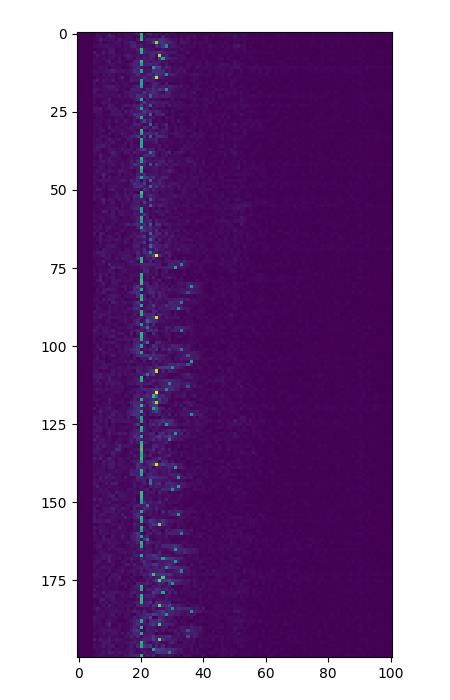
\includegraphics[width=\textwidth]{waterfall_sync_clean.png}
        \caption{Clean signal}
    \end{subfigure}
    \begin{subfigure}{0.45\textwidth}
        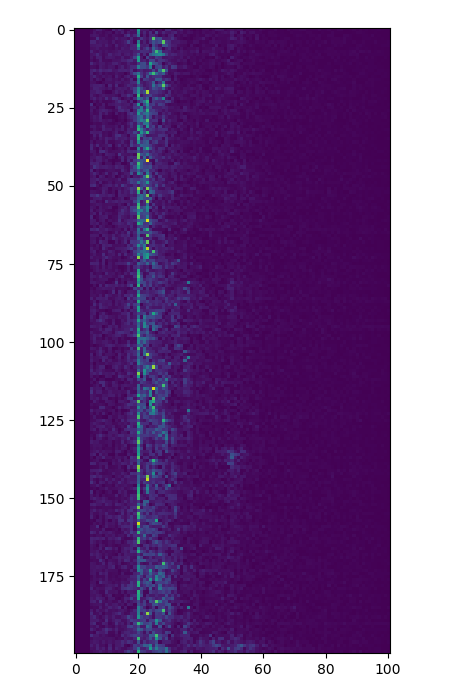
\includegraphics[width=1\textwidth]{waterfall_sync_multipath.png}
        \caption{Multipath-affected signal}
    \end{subfigure}
\end{figure}

Notice how the power creeps from one symbol to the next few one, and
blur the image, making correct demodulation impossible. This signal
cannot be decoded, despite having no significant noise in it.

The next images show correlation vectors of the same signals. The
correlation vector contains information about the position of the
received frame. The clean signal has a sharp, single spike with small
side lobes, whereas the multipath-affected signal has multiple large
bumps near the main spike that also looks flattened. This is a sign of
multiple synchronization vectors in the same audio. During the
experiment only one transmitter was used, so these must be different
copies of the very same signal bouncing around the room, and getting
back into the microphone.

\begin{figure}[H]
    \centering
    \begin{subfigure}{0.45\textwidth}
        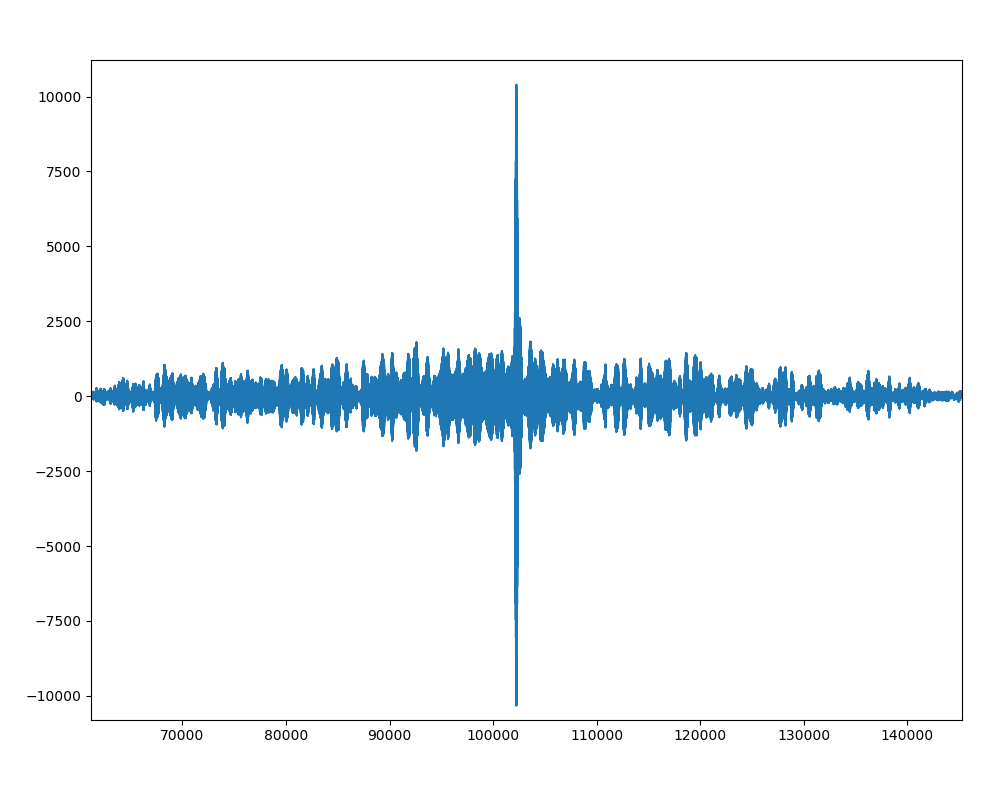
\includegraphics[width=1\textwidth]{correlation_clean.png}
        \caption{Correlation vector of a reasonably clean signal}
    \end{subfigure}
    \begin{subfigure}{0.45\textwidth}
        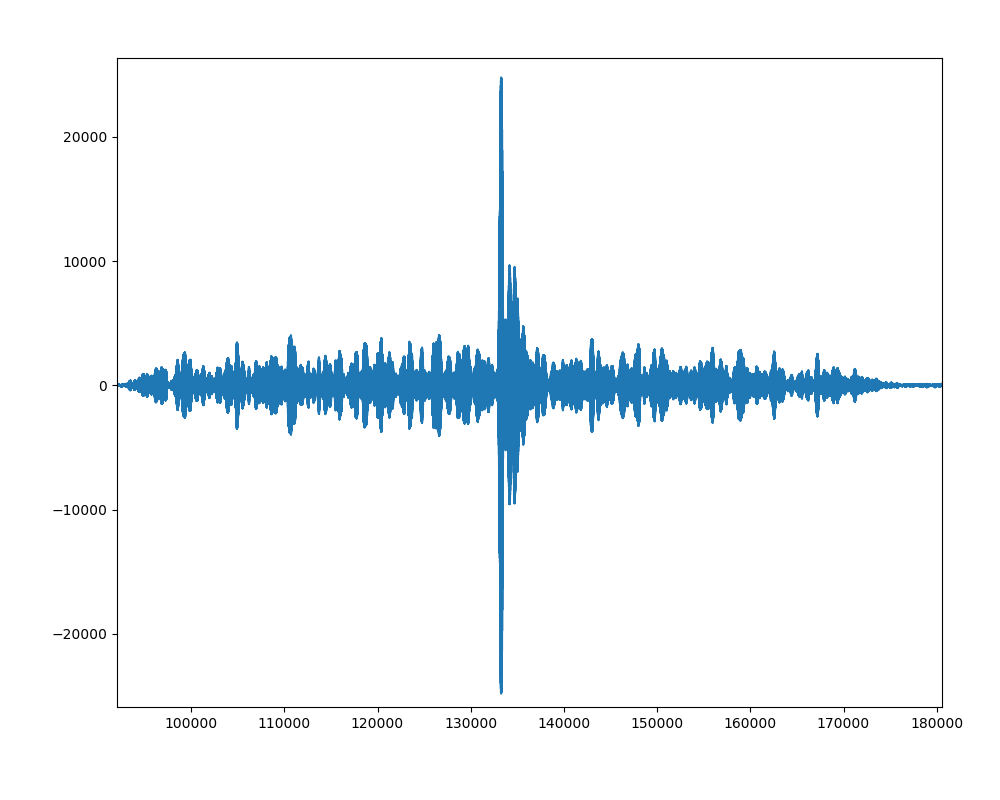
\includegraphics[width=1\textwidth]{correlation_multipath.png}
        \caption{Correlation vector of a signal affected by multipath}
    \end{subfigure}
\end{figure}

This problem were almost only encountered when the transmitting speaker
and the receiving microphone weren't facing each other. Microphones and
speakers tend to be directional \emph{by design}. If they are facing
each other, they amplify the signal, and signals coming from other
directions are attenuated. If they are facing away each other, stray
signals are amplified, and the original one gets attenuated.

This phenomenon can be mitigated by increasing the symbol time, and
even by introducing guard intervals. This decreases symbol rate, and
makes synchronization harder. Using frequency hopping spread spectrum
(FHSS) is an other effective way to combat this issue.

\textbf{To tackle this problem efficiently, more information on the
transmitting equipment and the working environments is needed, because
the carrier frequency, bandwidth, noise, and multipath models need to be
gotten right for the design of the system to be optimal.}

\begin{thebibliography}{9}
\bibitem{sox1}
  SoX, \url{http://sox.sourceforge.net/}
\bibitem{ana1}
  Anaconda, \url{https://www.anaconda.com/download}
\bibitem{ft1}
  Steven J. Franke, K9AN and Joseph H. Taylor, K1JT
  \emph{Open Source Soft-Decision Decoder for the JT65 (63,12) Reed-Solomon
  Code}, QEX, 2016
\end{thebibliography}


\end{document}
